\documentclass[fleqn,amsmath,amssymb,superscriptaddress, reprint,prl]{revtex4-1}
\usepackage{graphicx} %include figure files
\usepackage{dcolumn} %align table columns on decimal point (?)
\usepackage{bm} %bold math
\usepackage{hyperref} %add hypertext capabilities
\usepackage{longtable} % for tables with figures
\usepackage[T1]{fontenc}
\usepackage{times}
\usepackage{lipsum}
\usepackage{xcolor}
\usepackage{enumitem}
\usepackage{outlines}
\graphicspath{{figures/} }
\renewcommand{\UrlFont}{\small}
\newcommand\red[1]{\textcolor{red}{#1}}
\newcommand\blue[1]{\textcolor{blue}{#1}}
\newcommand\purple[1]{\textcolor{purple}{#1}}
\newcommand{\eg} {\textit{e.g.} }
\newcommand{\ie} {\textit{i.e.} }
\renewcommand{\figurename} {Figure}
\renewcommand{\thefigure} {\arabic{figure}}
\maxdeadcycles=200
\begin{document}


\begin{figure}
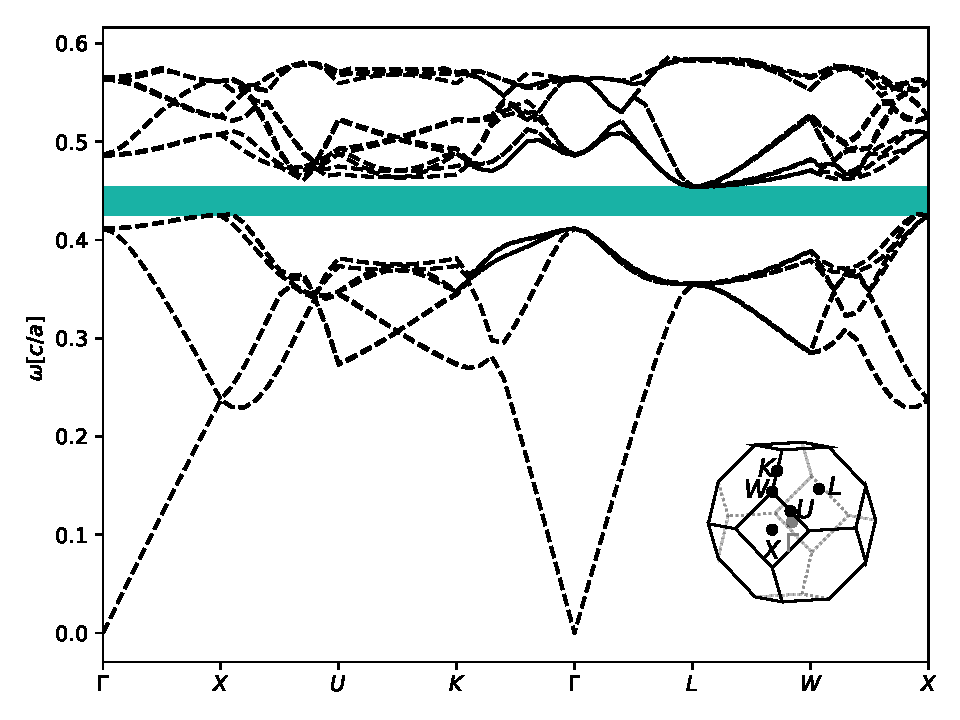
\includegraphics[width=0.9\linewidth]{workspace/38198cf16cc5ca53f90667fddd901139/images/r=11.pdf}
	\caption{\textbf{Aluminum Fluoride ($cF$288-AlH\textsubscript{2}\textsubscript{.}\textsubscript{2}\textsubscript{5}O\textsubscript{1}\textsubscript{.}\textsubscript{8}\textsubscript{7}\textsubscript{5}F\textsubscript{1}\textsubscript{.}\textsubscript{5}) at $\phi=0.38$}. 6.45\% gap between bands 8-9.}
\end{figure}
\end{document}